\section{Results Discussion}
\label{sec:discussion}


discussion on performance results.  discussion on energy results.  discussion on
nergy-delay product using Figure~\ref{fig:overall}.
\begin{figure*}[h]
	\centering
	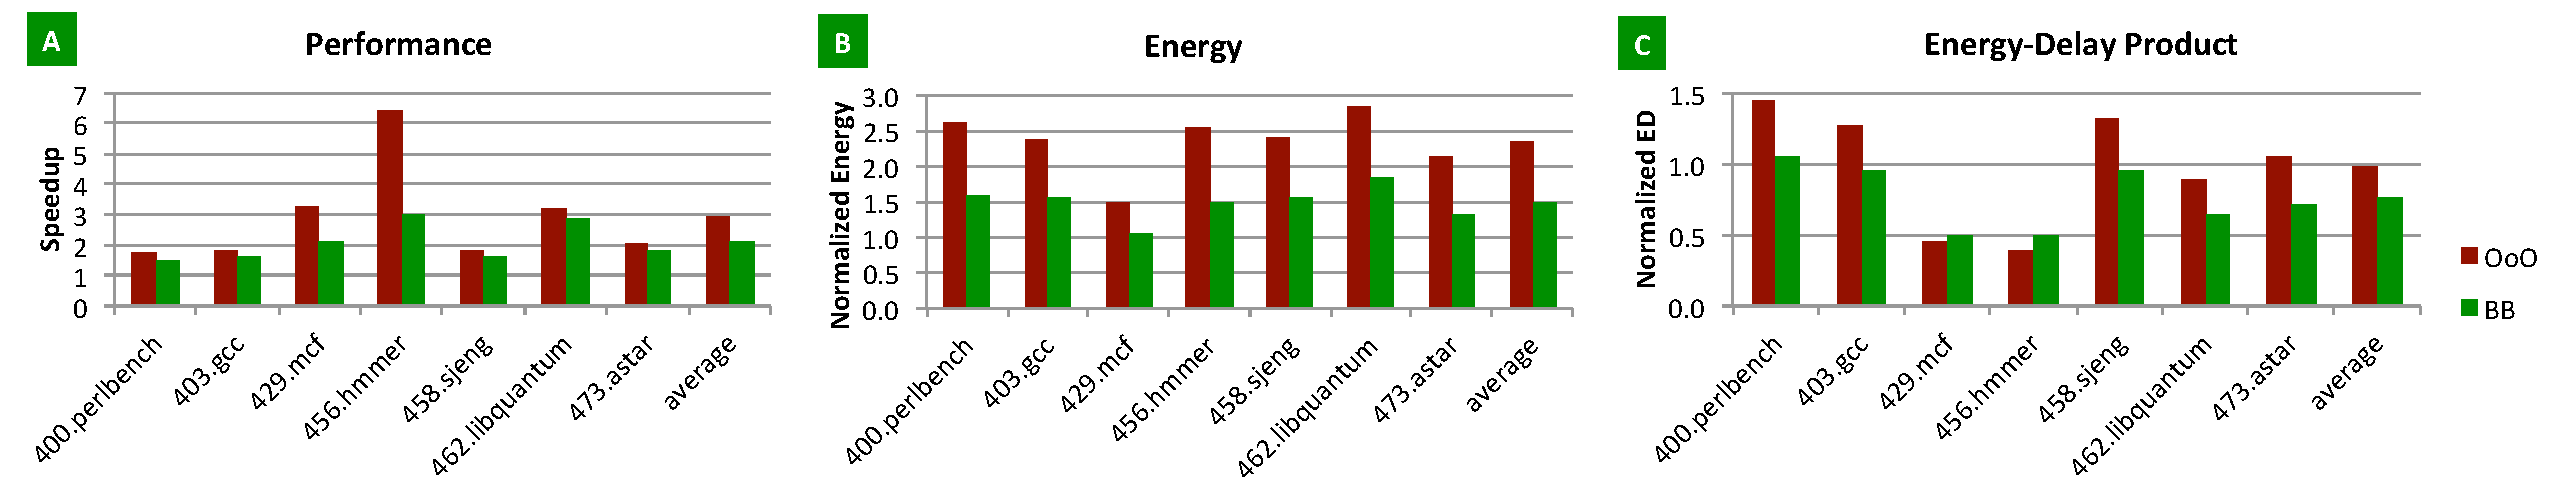
\includegraphics[width=\textwidth]{result/overall_perf.pdf} 
    \caption{(A) $IPC_{CORE}/IPC_{BASE}$, (B) $E_{CORE}/E_{BASE}$, (C)
        $ED_{CORE}/ED_{BASE}$; $CORE$ refers to BB and OoO and $BASE$ refers to
            INO core.}
	\label{fig:overall}
\end{figure*}

sweep of bbWindows sizes Figure~\ref{fig:bbWin_size}.
\begin{figure}[h]
	\centering
	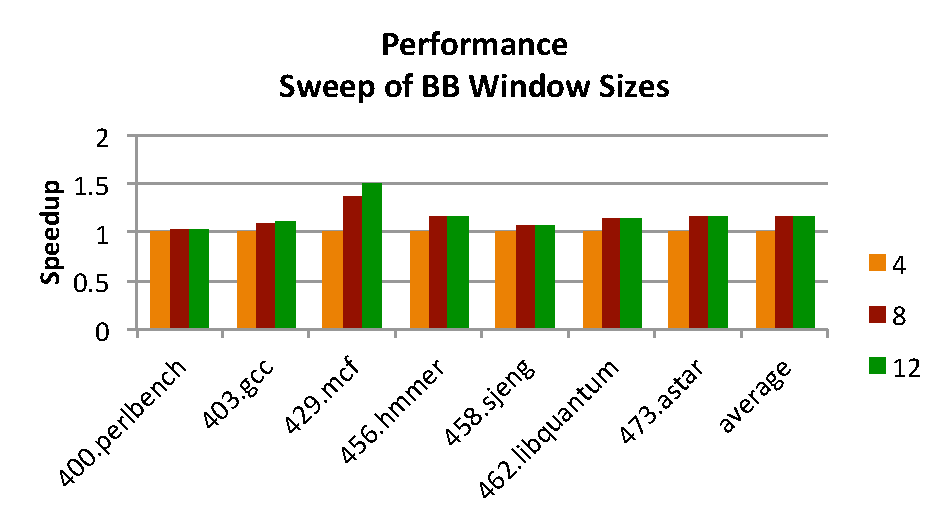
\includegraphics[width=1.0\columnwidth]{result/bbWin_size.pdf} 
    \caption{Performance \& energy change with sweeping the BB Window FIFO queue size}
	\label{fig:bbWin_size}
\end{figure}

evaluate the effect of multi-ins issue per BB. Figure~\ref{fig:bbWin_ins_cnt}
\begin{figure}[h]
	\centering
	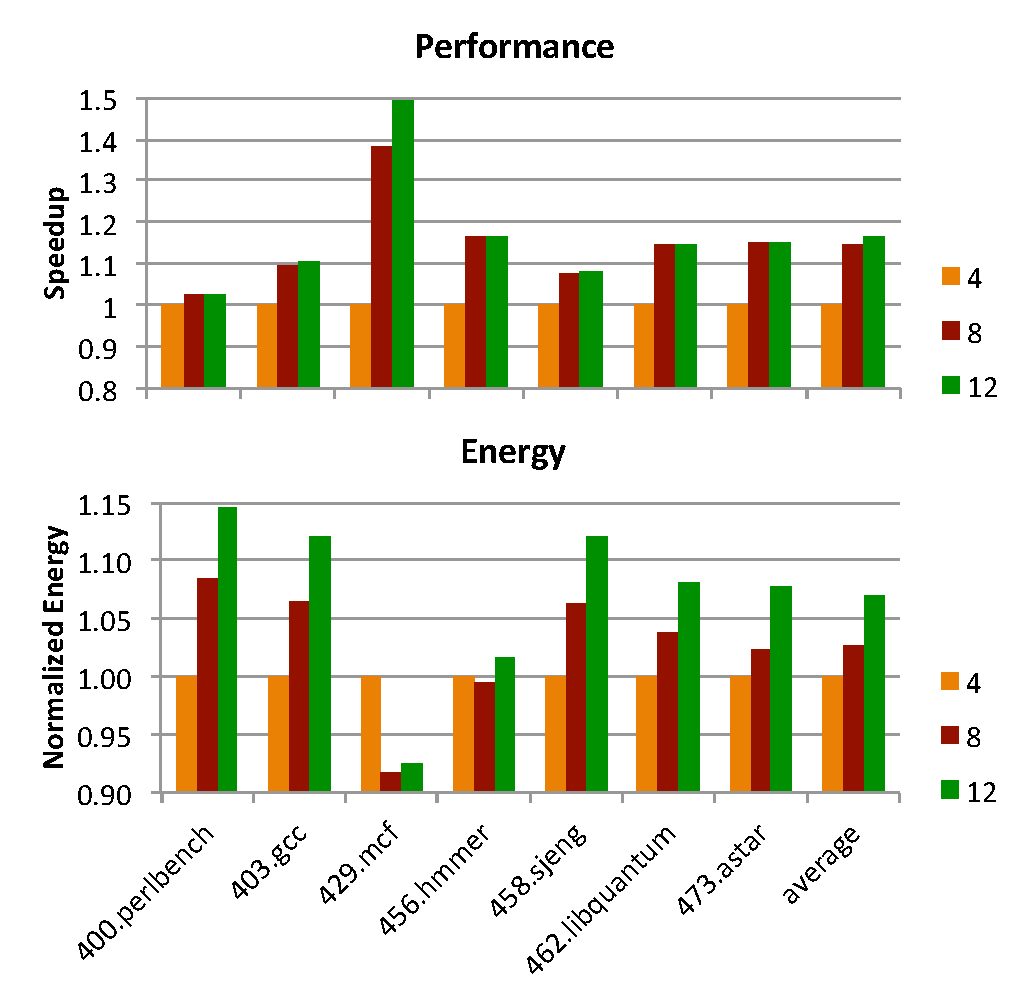
\includegraphics[width=1.0\columnwidth]{result/bbWin_ins_cnt.pdf} 
    \caption{Performance \& energy change with sweeping the number of BB Windows}
	\label{fig:bbWin_ins_cnt}
\end{figure}

evaluation of LRF and no LRF on performance and energy. Figure~\ref{fig:lrf_effect}
\begin{figure}[h]
	\centering
	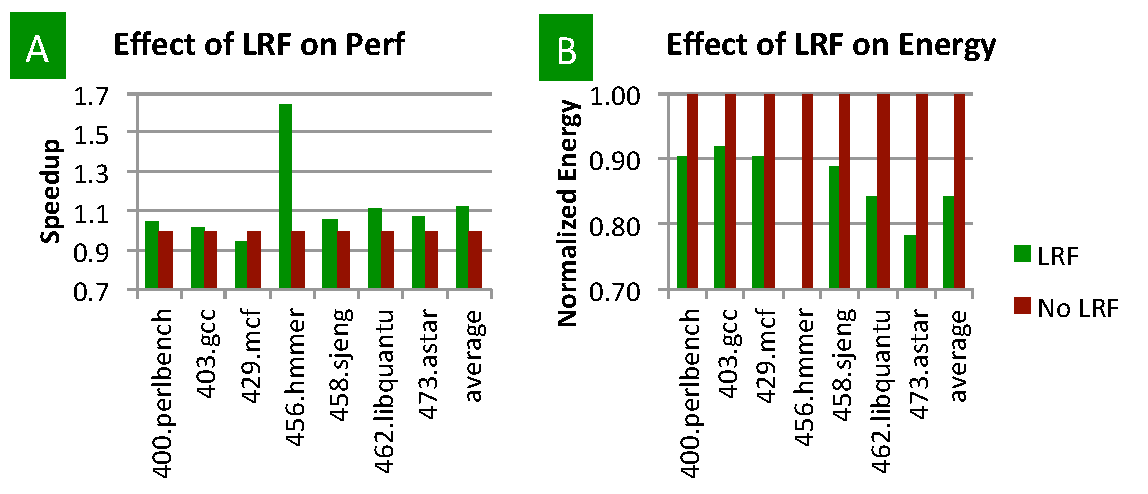
\includegraphics[width=1.0\columnwidth]{result/lrf_effect.pdf} 
    \caption{Performance \& energy change with sweeping the number of BB Windows}
	\label{fig:lrf_effect}
\end{figure}

evaluate the effect of multi-ins issue per BB. Figure~\ref{fig:bbWin_port}
\begin{figure}[h]
	\centering
	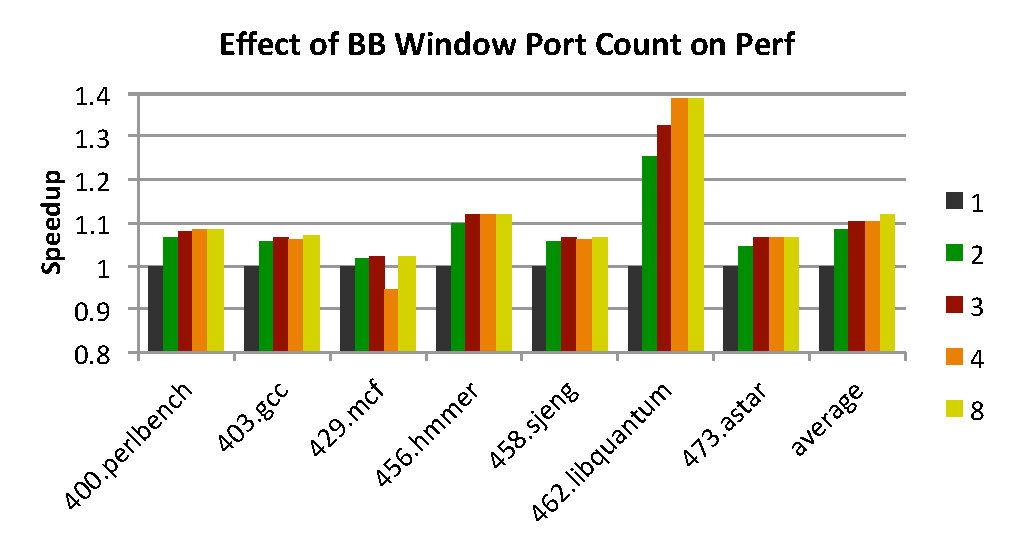
\includegraphics[width=1.0\columnwidth]{result/bbWin_port.pdf} 
    \caption{Performance \& energy change with sweeping the number of BB Window
    ports}
	\label{fig:bbWin_port}
\end{figure}

sweep of register file sizes. 

various numbers for EU's. Figure~\ref{fig:ep}
\begin{figure}[h]
	\centering
	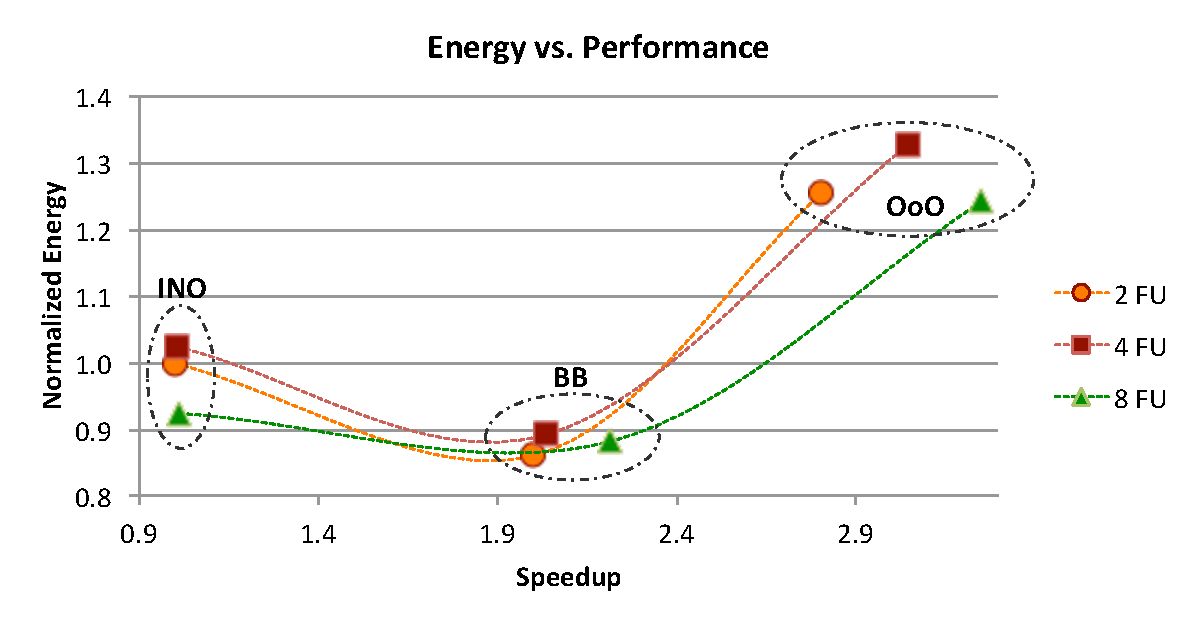
\includegraphics[width=1.0\columnwidth]{result/ep.pdf} 
    \caption{Energy vs. Performance Trend for OoO, BB, \& InO}
	\label{fig:ep}
\end{figure}


evaluation of pipeline stages.

forwarding support ability. Figure~\ref{fig:forwarding}
\begin{figure}[h]
	\centering
	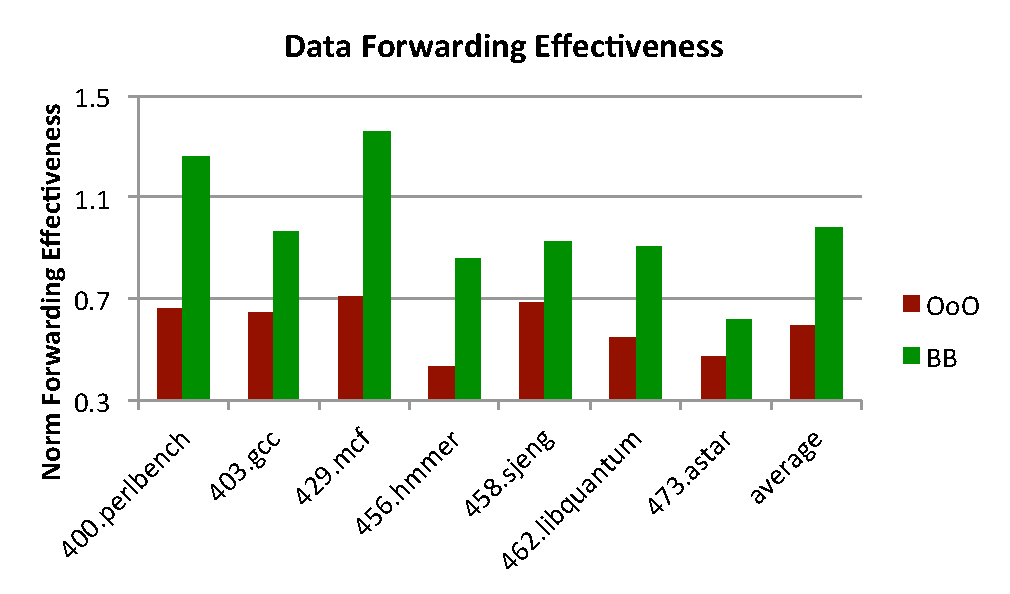
\includegraphics[width=1.0\columnwidth]{result/forwarding.pdf} 
    \caption{Energy vs. Performance Trend for OoO, BB, \& InO}
	\label{fig:forwarding}
\end{figure}

BPU activity and energy.
area evaluation.

%comparison of new and conventional register rename model.
%comparison of new and conventional squash mode.

